\chapter*{Questão 2}

{\it Implemente o método dos mínimos quadrados offline e teste o programa com o
processo da questão 1. simulando variações lentas em seus parâmetros ($\pm
10\%$) e avaliando o comportamento das estimativas.}

{\it Apresente gráficos mostrando as estimativas, os valores reais dos
parâmetros, o sinal de controle, a saída real e a estimada com cada modelo
utilizado.}

\vspace{0.5cm}

\noindent{\bf Resolução:}

\vspace{0.25cm}

O sistema da questão 1. consiste na função de transferência dada pela Eq.
\ref{eq:sist}:

\begin{equation}\label{eq:sist}
G(s) = \frac{Y(s)}{U(s)} = \frac{0.5}{(s + 0.5)(s + 1)}
\end{equation}

A discretização obtida nessa mesma questão é repetida pela Eq.
\ref{eq:sist_disc},

\begin{equation}\label{eq:sist_disc}
y(k) - 1.7235y(k-1) + 0.7408k(k-2) = 0.0091u(k-1) + 0.0082u(k-2)
\end{equation}

Generalizando o modelo obtido na Eq. \ref{eq:sist_disc} e isolando o termo
$y(k)$, tem-se que:

\begin{eqnarray}
y(k) + a_1 y(k-1) + a_2 y(k-2) = b_1 u(k-1) + b_2 u(k-2)\nonumber\\
y(k) = - a_1 y(k-1) - 
         a_2 y(k-2) + 
         b_1 u(k-1) + 
         b_2u(k-2)\label{eq:eq_a_dif_geral}
\end{eqnarray}

O estimador de mínimos quadrados não-recursivo considera um sistema representado
por uma equação a diferenças semelhante a Eq. \ref{eq:eq_a_dif_geral}. Segundo
\citeasnoun{coelho:2004}, haverão $n_a + n_b + 1$ parâmetros a serem estimados
pelo algoritmo e para determinar os valores de $a_i$, deve-se utilizar as
medidas de entrada e saída do processo.

Assim sendo, de posse da equação generalizada dos parâmetros do sistema,
utilizar o método dos mínimos quadrados {\it offline} consiste em excitar a
planta com um determinado sinal de entrada e armazenar os valores de saída
obtidos para executar o algoritmo não-recursivo. Assim sendo, pode-se dizer que
o processo de identificação é realizado de uma só vez, ou em batelada.

Supondo que exista um sistema discreto que possa ser descrito conforme {\it
modelo de regressão linear}:

\begin{equation}\label{eq:mode_reg_lin}
\mb{Y} = \mb{X\theta} + \mb{e}
\end{equation}

\noindent tal que $\mb{Y}$ corresponde à saída do sistema, $\mb{X}$ é um vetor
determinístico conhecido, $\mb{\theta}$ é o vetor de parâmetros a serem
estimados e $\mb{e}$ corresponde ao erro do modelo. Deseja-se então, estimar o
vetor $\mb{\theta}$ a partir de $N$ experimentos, de tal forma que:

\begin{eqnarray}
\mb{Y}_1 & = & \mb{X}_1\mb{\theta}_1 + \mb{e}_1\nonumber\\
\mb{Y}_2 & = & \mb{X}_2\mb{\theta}_2 + \mb{e}_2\nonumber\\
& & \vdots\nonumber\\ 
\mb{Y}_N & = & \mb{X}_N\mb{\theta}_N + \mb{e}_N\nonumber
\end{eqnarray}

\noindent considerando:

\begin{equation*}
\mb{\theta} = \left[
\begin{array}{c}
a_1\\
a_2\\
\vdots\\
a_n\\
\hline
b_1\\
b_2\\
\vdots\\
b_m
\end{array}
\right] \qquad
\mb{X} = \left[
\begin{array}{cccc}
-Y(1) & -Y(0) & u(1) & u(0)\\
-Y(2) & -Y(1) & u(2) & u(1)\\
\vdots & \vdots & \vdots & \vdots\\
-Y(N-1) & -Y(N-n) & u(N-1) & u(N-m)
\end{array}
\right]
\end{equation*}

\begin{equation*}
\mb{Y} = \left[
\begin{array}{c}
y_1\\
y_2\\
\vdots\\
y_N
\end{array}
\right] \qquad
\mb{e} = \left[
\begin{array}{c}
e_1\\
e_2\\
\vdots\\
e_N
\end{array}
\right]
\end{equation*}

O método dos mínimos quadrados tem por objetivo realizar a estimativa de
$\mb{\theta}$ de modo a minimizar a função de erro $J$, tal que:

\begin{equation}
J = \sum_{K = 1}^N e^2(K) = \mb{e}^T\mb{e}
\end{equation}

Pela Eq. \ref{eq:mode_reg_lin}:

\begin{equation}
\mb{Y} = \mb{X\theta} + \mb{e} \quad\Longrightarrow\quad \mb{e} = \mb{Y} - \mb{X\theta}
\end{equation}

Assim, a função de erro $J$, pode ser reescrita como:

\begin{equation}\label{eq:J}
J = (\mb{Y} - \mb{X\theta})^T(\mb{Y} - \mb{X\theta})
\end{equation}

\noindent que possui mínimo quando:

\begin{equation*}
\left.\frac{\partial J}{\partial \theta}\right|_{\theta = \hat{\mb{\theta}}} = 0
\end{equation*}

Considerando que:

\begin{equation*}
\frac{\partial (\mb{Ax} + \mb{b})^T\mb{C}(\mb{Dx} + \mb{e})}{\partial \mb{x}} =
(\mb{Dx} + \mb{e})^T\mb{C}^T\mb{A} + (\mb{Ax} + \mb{b})^T\mb{CD}
\end{equation*}

\noindent e fazendo:

\begin{equation*}
\begin{array}{c@{\qquad}c@{\qquad}c}
\mb{A} = -\mb{X} & \mb{x} = \mb{\theta} & \mb{b} = \mb{Y}\\
\mb{C} = \mb{I}  & \mb{D} = -\mb{X}     & \mb{e} = \mb{Y}
\end{array}
\end{equation*}

\noindent na Eq. \ref{eq:J}, tem-se que:

\begin{eqnarray}
\frac{\partial J}{\partial \mb{\theta}} & = & 
(-\mb{X\theta}+\mb{Y})^T(-\mb{X}) + (-\mb{X\theta}+\mb{Y})^T(-\mb{X})\nonumber\\
& = & -2 \left[(-\mb{X\theta}+\mb{Y})\right]^T\mb{X}\nonumber\\
& = & -2 \left[(-\mb{X\theta})^T + \mb{Y}^T\right]\mb{X}\nonumber\\
& = & -2 \left[-\mb{\theta}^T\mb{X}^T + \mb{Y}^T\right]\mb{X}\nonumber\\
& = & 2 \mb{\theta}^T\mb{X}^T\mb{X} -2 \mb{Y}^T\mb{X}\label{eq:deduc}
\end{eqnarray}

Como $\D\frac{\partial J}{\partial \mb{\theta}} = 0$ (escalar), então,
pode-se transpor a Eq. \ref{eq:deduc}, de tal forma que:

\begin{eqnarray}
\frac{\partial J}{\partial \mb{\theta}} & = & 
2\mb{X}^T(\mb{\theta}^T\mb{X}^T)^T - 2\mb{X}^T\mb{Y}\nonumber\\
0 & = & 2\mb{X}^T(\mb{X\theta}) - 2\mb{X}^T\mb{Y}\nonumber\\
0 & = & 2\mb{X}^T\mb{X\theta} - 2\mb{X}^T\mb{Y}
\end{eqnarray}

Substituindo $\mb{\theta}$ por $\hat{\mb{\theta}}$ e isolando
$\hat{\mb{\theta}}$, tem-se que:

\begin{equation}\label{eq:theta_est}
\hat{\mb{\theta}} = (\mb{X}^T\mb{X})^{-1} \mb{X}^T\mb{Y}
\end{equation}

Algumas observações podem ser feitas acerca da Eq. \ref{eq:theta_est}:

\begin{itemize}
    \item A solução existirá quando $(\mb{X}^T\mb{X})^{-1}$ for não singular
    \item A sequência escolhida das entradas $u(k)$ deverá garantir essa
          não singularidade
    \item Quando não há a presença de ruídos $\hat{\mb{\theta}}$ pode ser
          encontrado em $n+m$ passos
    \item A matriz $\mb{X}$ cresce na medida em que $N$ cresce
\end{itemize}

O algoritmo desenvolvido leva em consideração uma variação dos parâmetros
aleatória para $\pm 10\%$ do valor do parâmetro a ser modificado. O número de
variações também é aleatório, correspondendo a, no máximo, 5\% do número de
amostras. Ou seja, se forem consideradas 100 amostras, haverão, no máximo, $5-1
= 4$ variações de parâmetros equiespaçadas, uma vez que da primeira amostra até
a primeira variação não deve ser contabilizada. A variação dos parâmetros é
mantida até que um novo valor seja sorteado.

O sinal de entrada do sistema varia de maneira análoga à variação dos parâmetros
da função, ou seja, a cada $K$ iterações o sinal muda e se mantém naquele valor
até o próximo instante de variação. Para compor esse sinal, o número máximo de
variações correspondia a 50\% do número de amostras. O valor da entrada $u(k)$
variava entre $\pm 50\%\ u(k-1)$ nos instantes de variação e era repetido para as
demais amostras.

No primeiro teste, foram consideradas 100 amostras. O número de variações
sorteado foi de 2 variações. Portanto, cada variação era mantida por 33
amostras. A saída do sistema com os parâmetros reais, bem como com os parâmetros
variáveis e o sinal de controle pode ser observada na Fig.
\ref{fig:saida_sist_100}. A estimativa realizada é vista na Tab.
\ref{tab:estimativa_100}.\footnote{Por questões de precisão, os valores
utilizados em todos os testes foram aqueles obtidos através do {\it script} do
MATLAB\textsuperscript{\textregistered} mostrado no Apêndice \ref{ap:q1_a}.}

\begin{figure}[htb]
\centering
    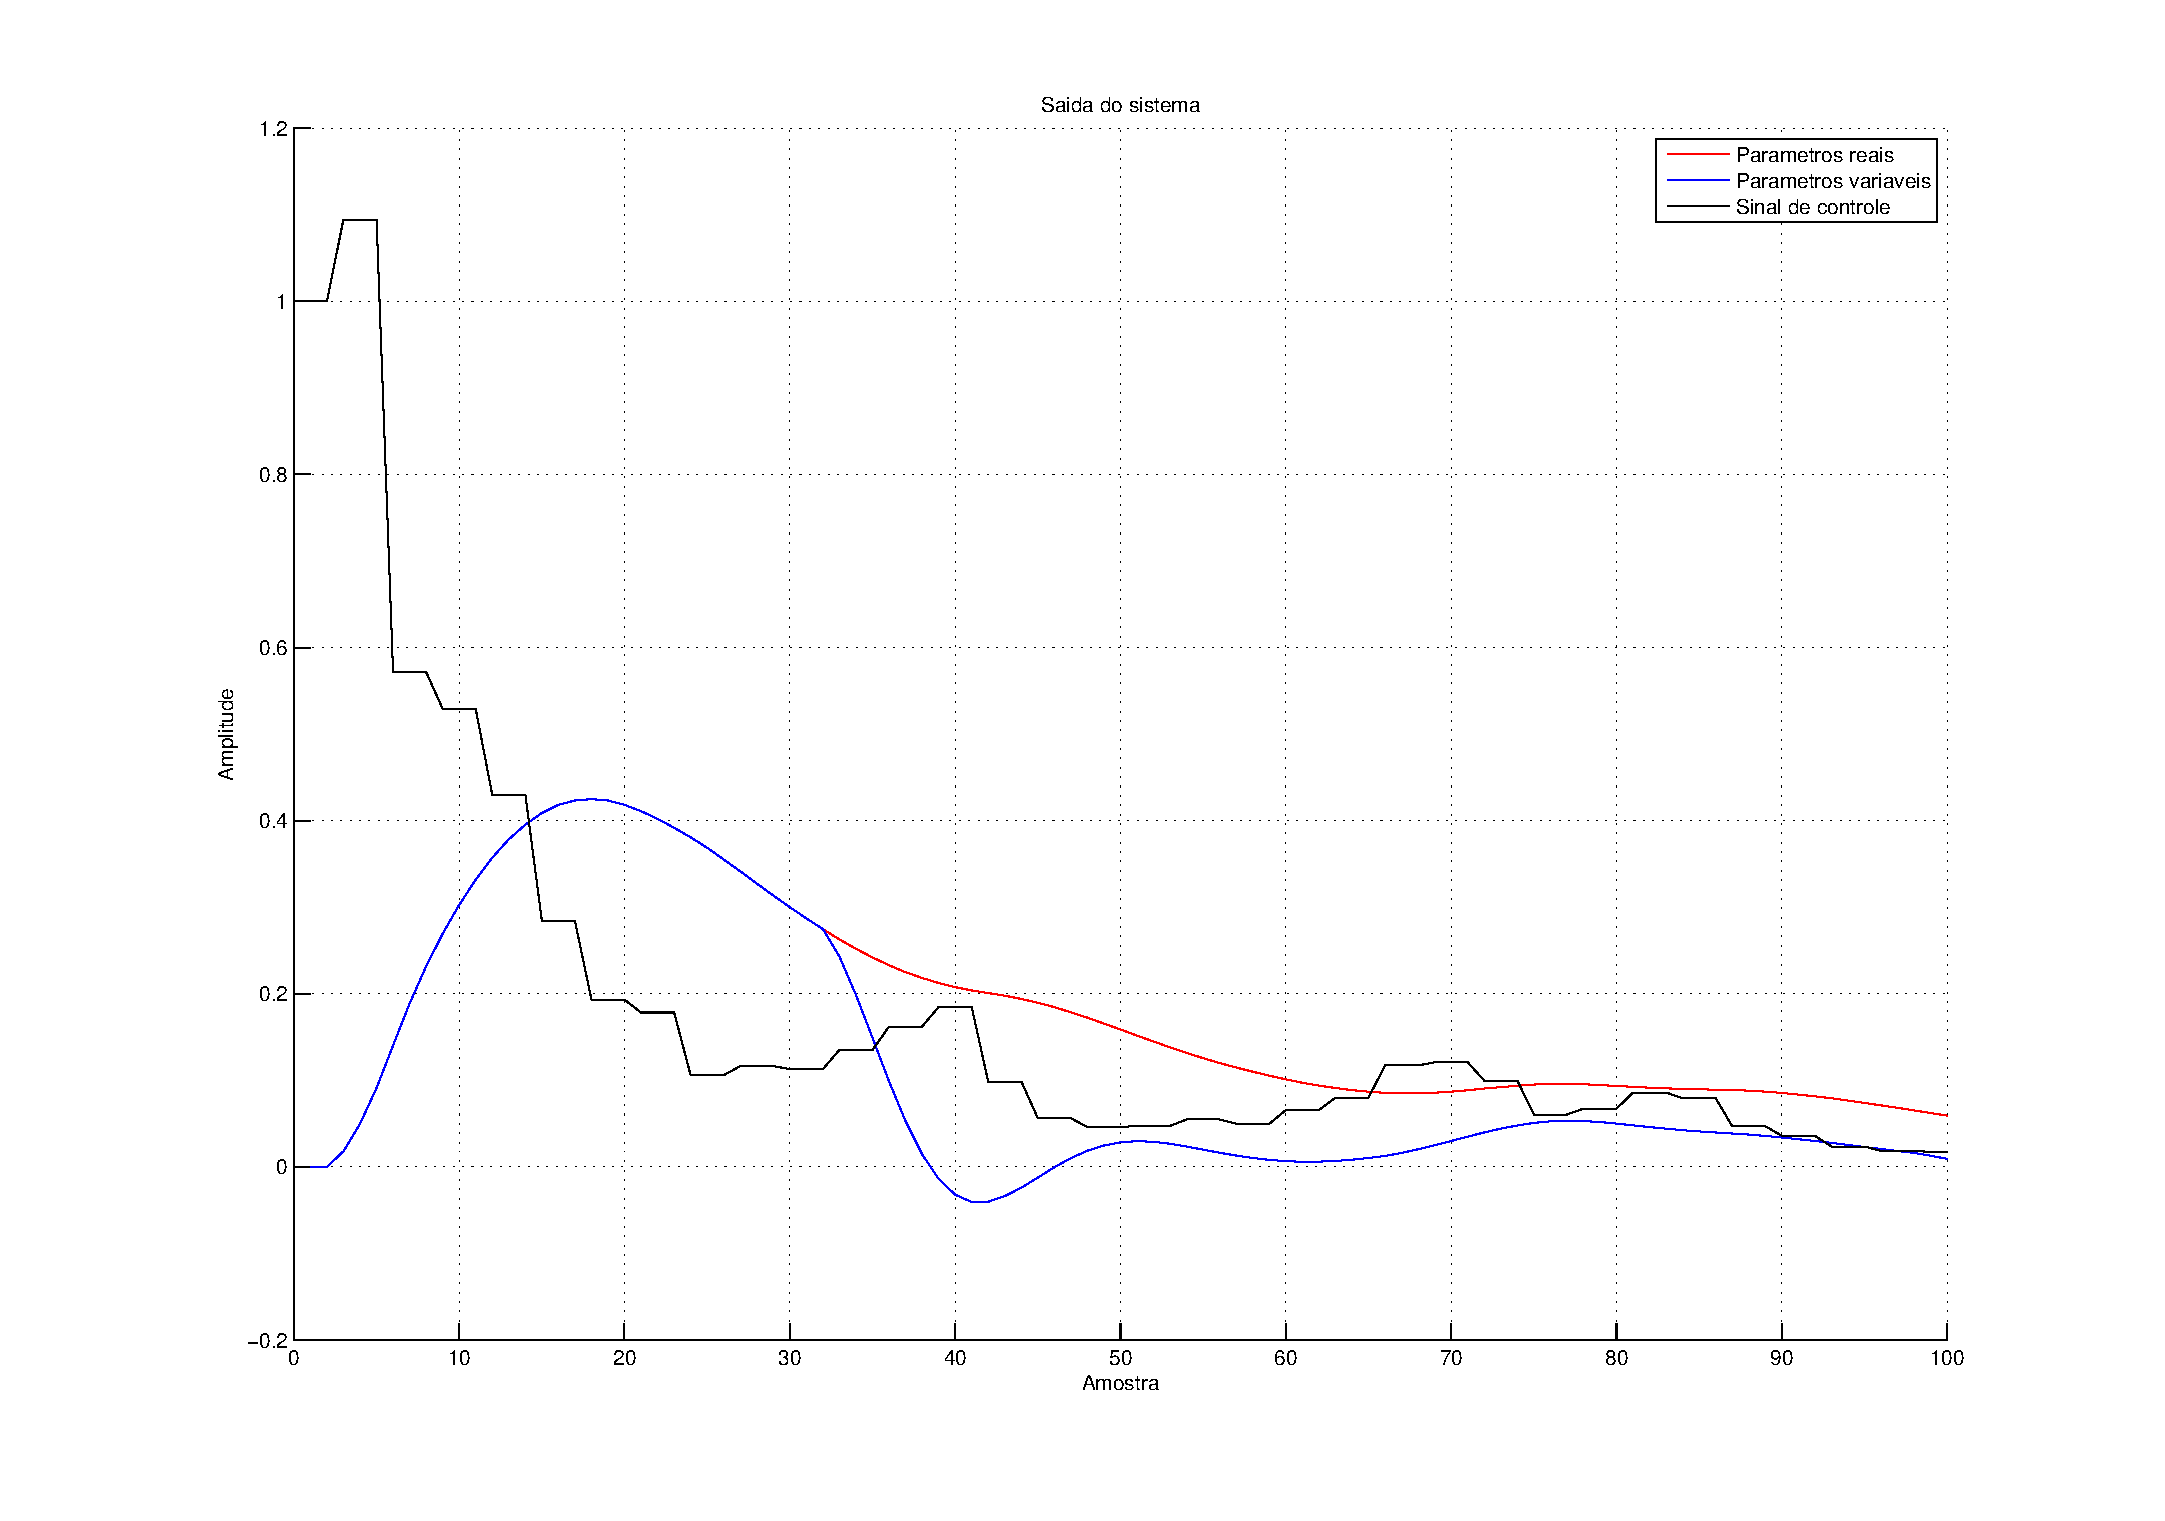
\includegraphics[width=0.95\textwidth]{imgs/questao2/saida_100}
    \caption{Saída do sistema para $N = 100$.}
    \label{fig:saida_sist_100}
\end{figure}

\begin{table}
\centering
    \caption{Estimativa realizada para $N = 100$.}
    \label{tab:estimativa_100}
    \vspace{0.25cm}
    \begin{tabular}{|c|c|c|c|}
        \hline
        Parâmetros & 
        $\mb{\theta}_{\text{ideal}}$&
        $\mb{\theta}_{\text{sem variação}}$&
        $\mb{\theta}_{\text{com variação}}$\\
        \hline
        \hline
        $a_1$ & $-1.724$   & $-1.7240$ & $-1.8617$ \\
        \hline
        $a_2$ & $0.7408$   & $0.7408$  & $0.8807$ \\
        \hline
        $b_1$ & $0.009056$ & $0.0096$  & $0.0103$ \\
        \hline
        $b_2$ & $0.008194$ & $0.0082$  & $0.0032$ \\
        \hline
    \end{tabular}
\end{table}

Devido a aleatoriedade envolvida no algoritmo, percebeu-se que quando há um
grande número de variações dos parâmetros ou quando a variação corresponde a um
valor elevado, o sistema se torna instável e sua saída passa a divergir, o que
leva a estimativas erradas dos parâmetros, como pode ser verificado na Fig.
\ref{fig:saida_sist_100_div} e na Tab. \ref{tab:estimativa_100_div}. Esses
resultados foram obtidos para 100 amostras e, coincidentemente, para 2
variações.

\begin{figure}[htb]
\centering
    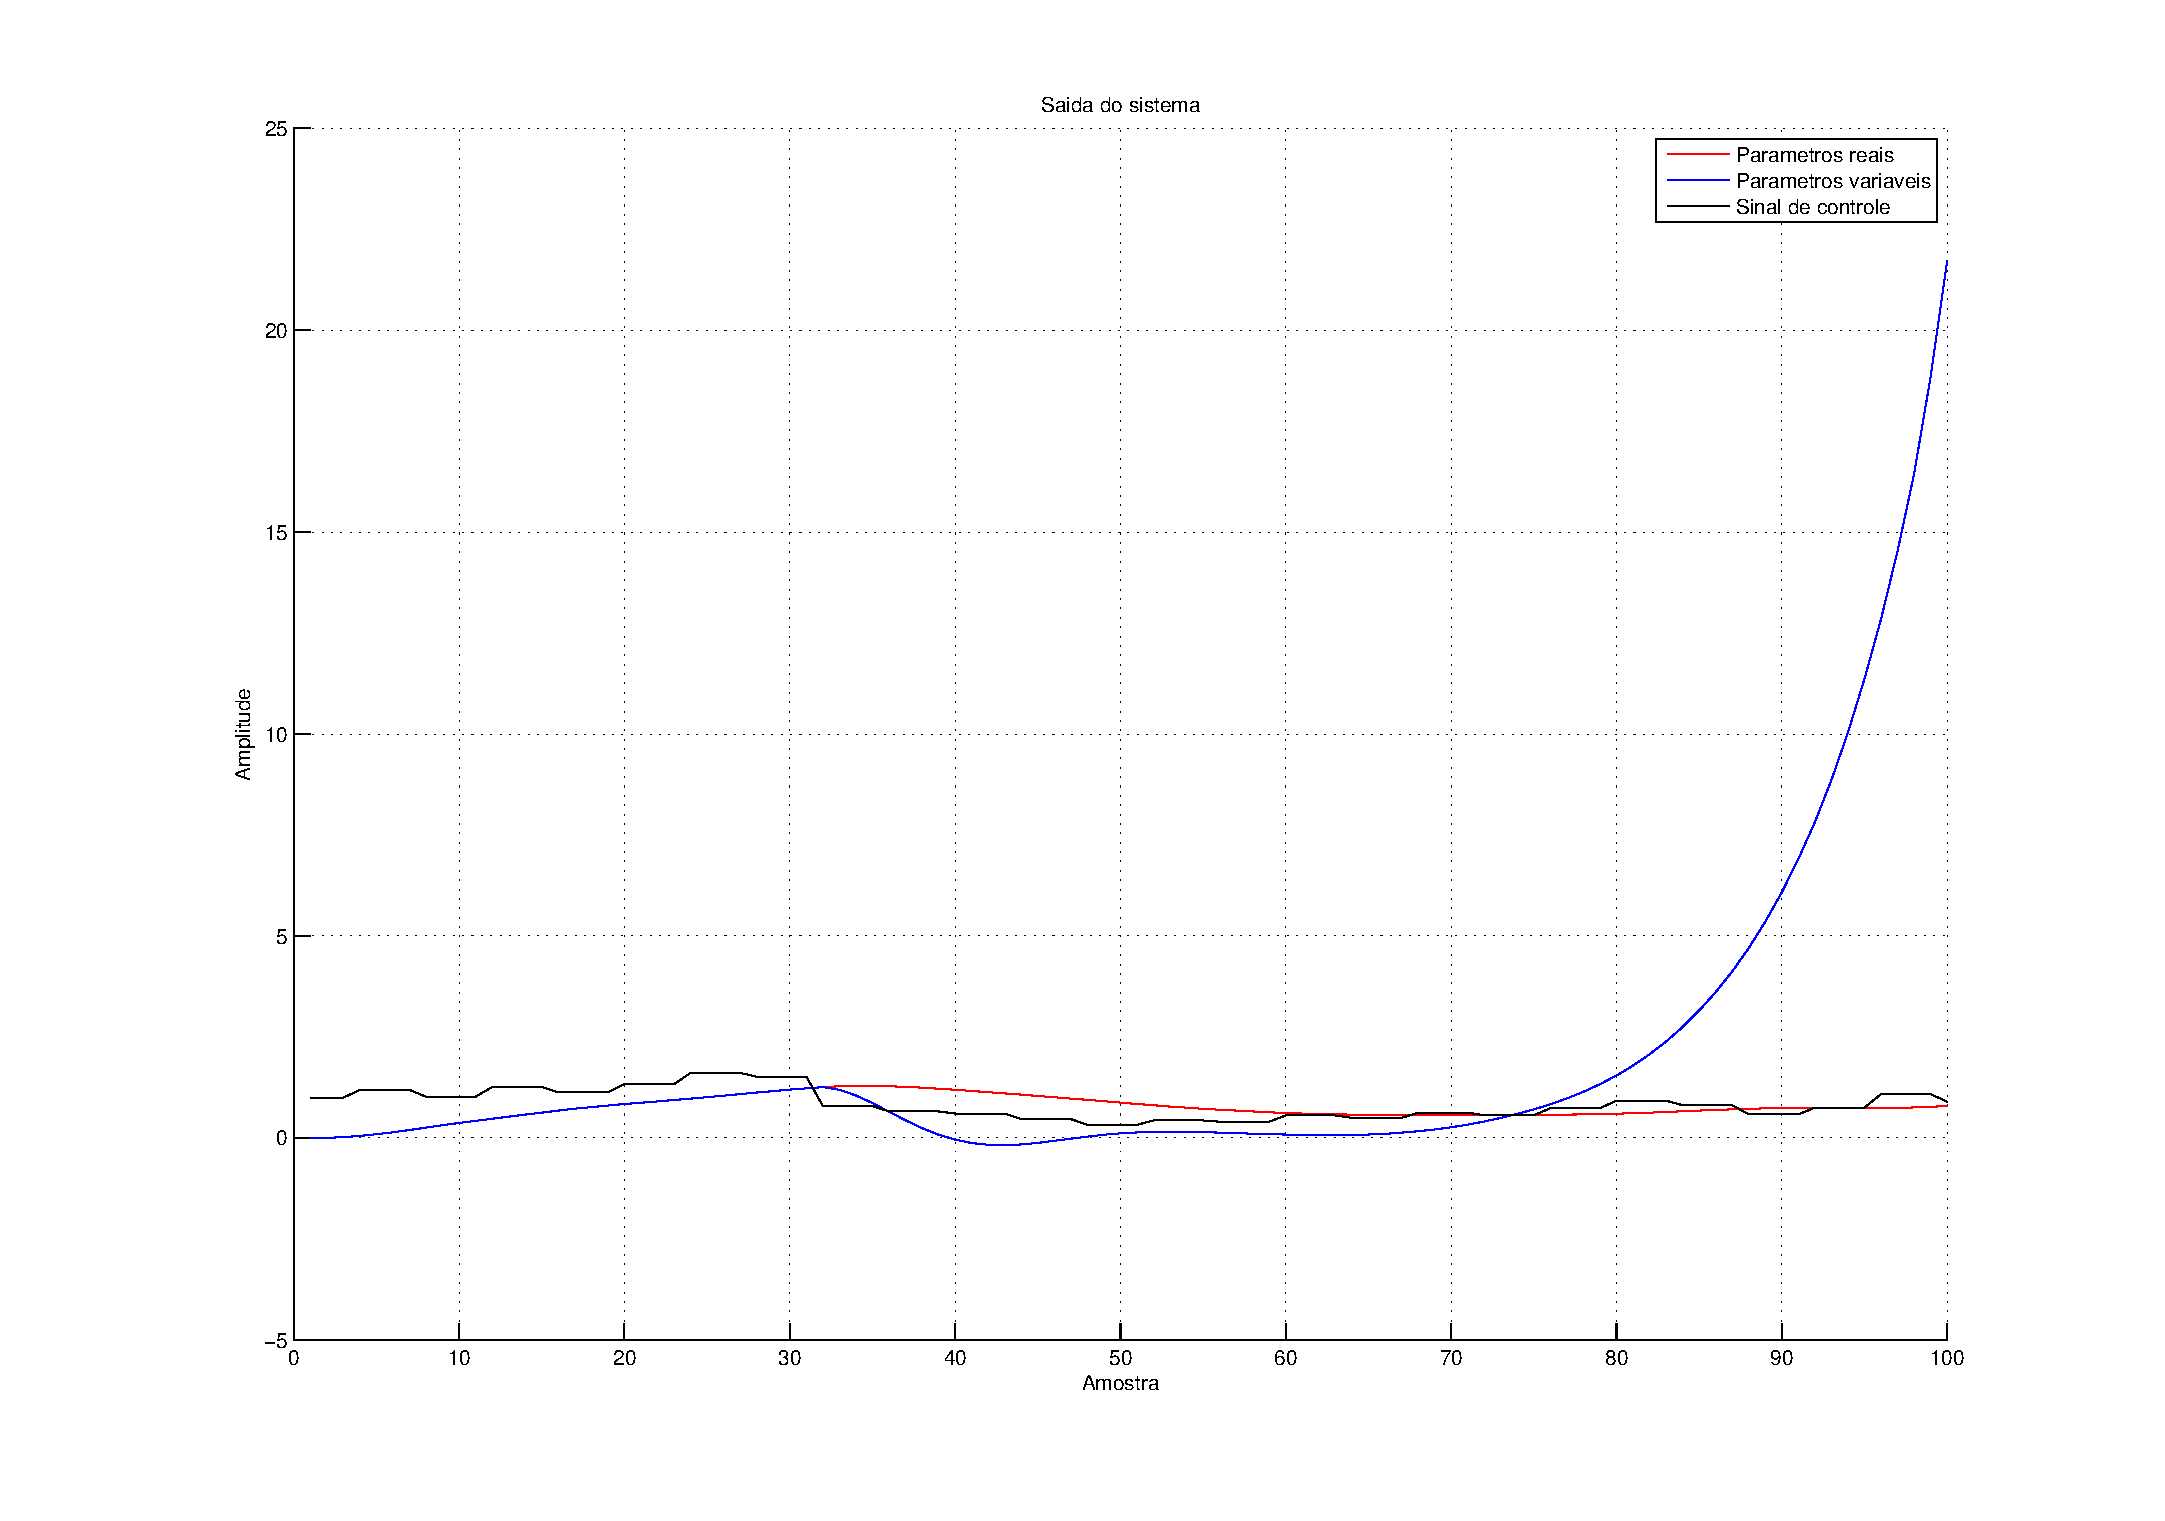
\includegraphics[width=0.95\textwidth]{imgs/questao2/saida_100_div}
    \caption{Saída do sistema para $N = 100$ -- Divergente.}
    \label{fig:saida_sist_100_div}
\end{figure}

\begin{table}
\centering
    \caption{Estimativa realizada para $N = 100$ -- Divergente.}
    \label{tab:estimativa_100_div}
    \vspace{0.25cm}
    \begin{tabular}{|c|c|c|c|}
        \hline
        Parâmetros & 
        $\mb{\theta}_{\text{ideal}}$&
        $\mb{\theta}_{\text{sem variação}}$&
        $\mb{\theta}_{\text{com variação}}$\\
        \hline
        \hline
        $a_1$ & $-1.724$   & $-1.7240$ & $-2,1177$ \\
        \hline
        $a_2$ & $0.7408$   & $0.7408$  & $1.1105$ \\
        \hline
        $b_1$ & $0.009056$ & $0.0096$  & $0.0400$ \\
        \hline
        $b_2$ & $0.008194$ & $0.0082$  & $-0.0463$ \\
        \hline
    \end{tabular}
\end{table}

O algoritmo também foi executado para 1000 amostras. Entranto, devido a
dificuldade de se encontrar valores de saída que não divergissem para o valor
máximo de 5\% do número de amostras de variações, ou seja, $50 - 1 = 49$
variações, essa porcentagem foi reduzida à 1\%. Os resultados obtidos para a
primeira execução podem ser observados na Fig. \ref{fig:saida_sist_1000} e na
Tab. \ref{tab:estimativa_1000}. Para esse resultado, houve apenas 1 variação dos
parâmetros.

\begin{figure}[htb]
\centering
    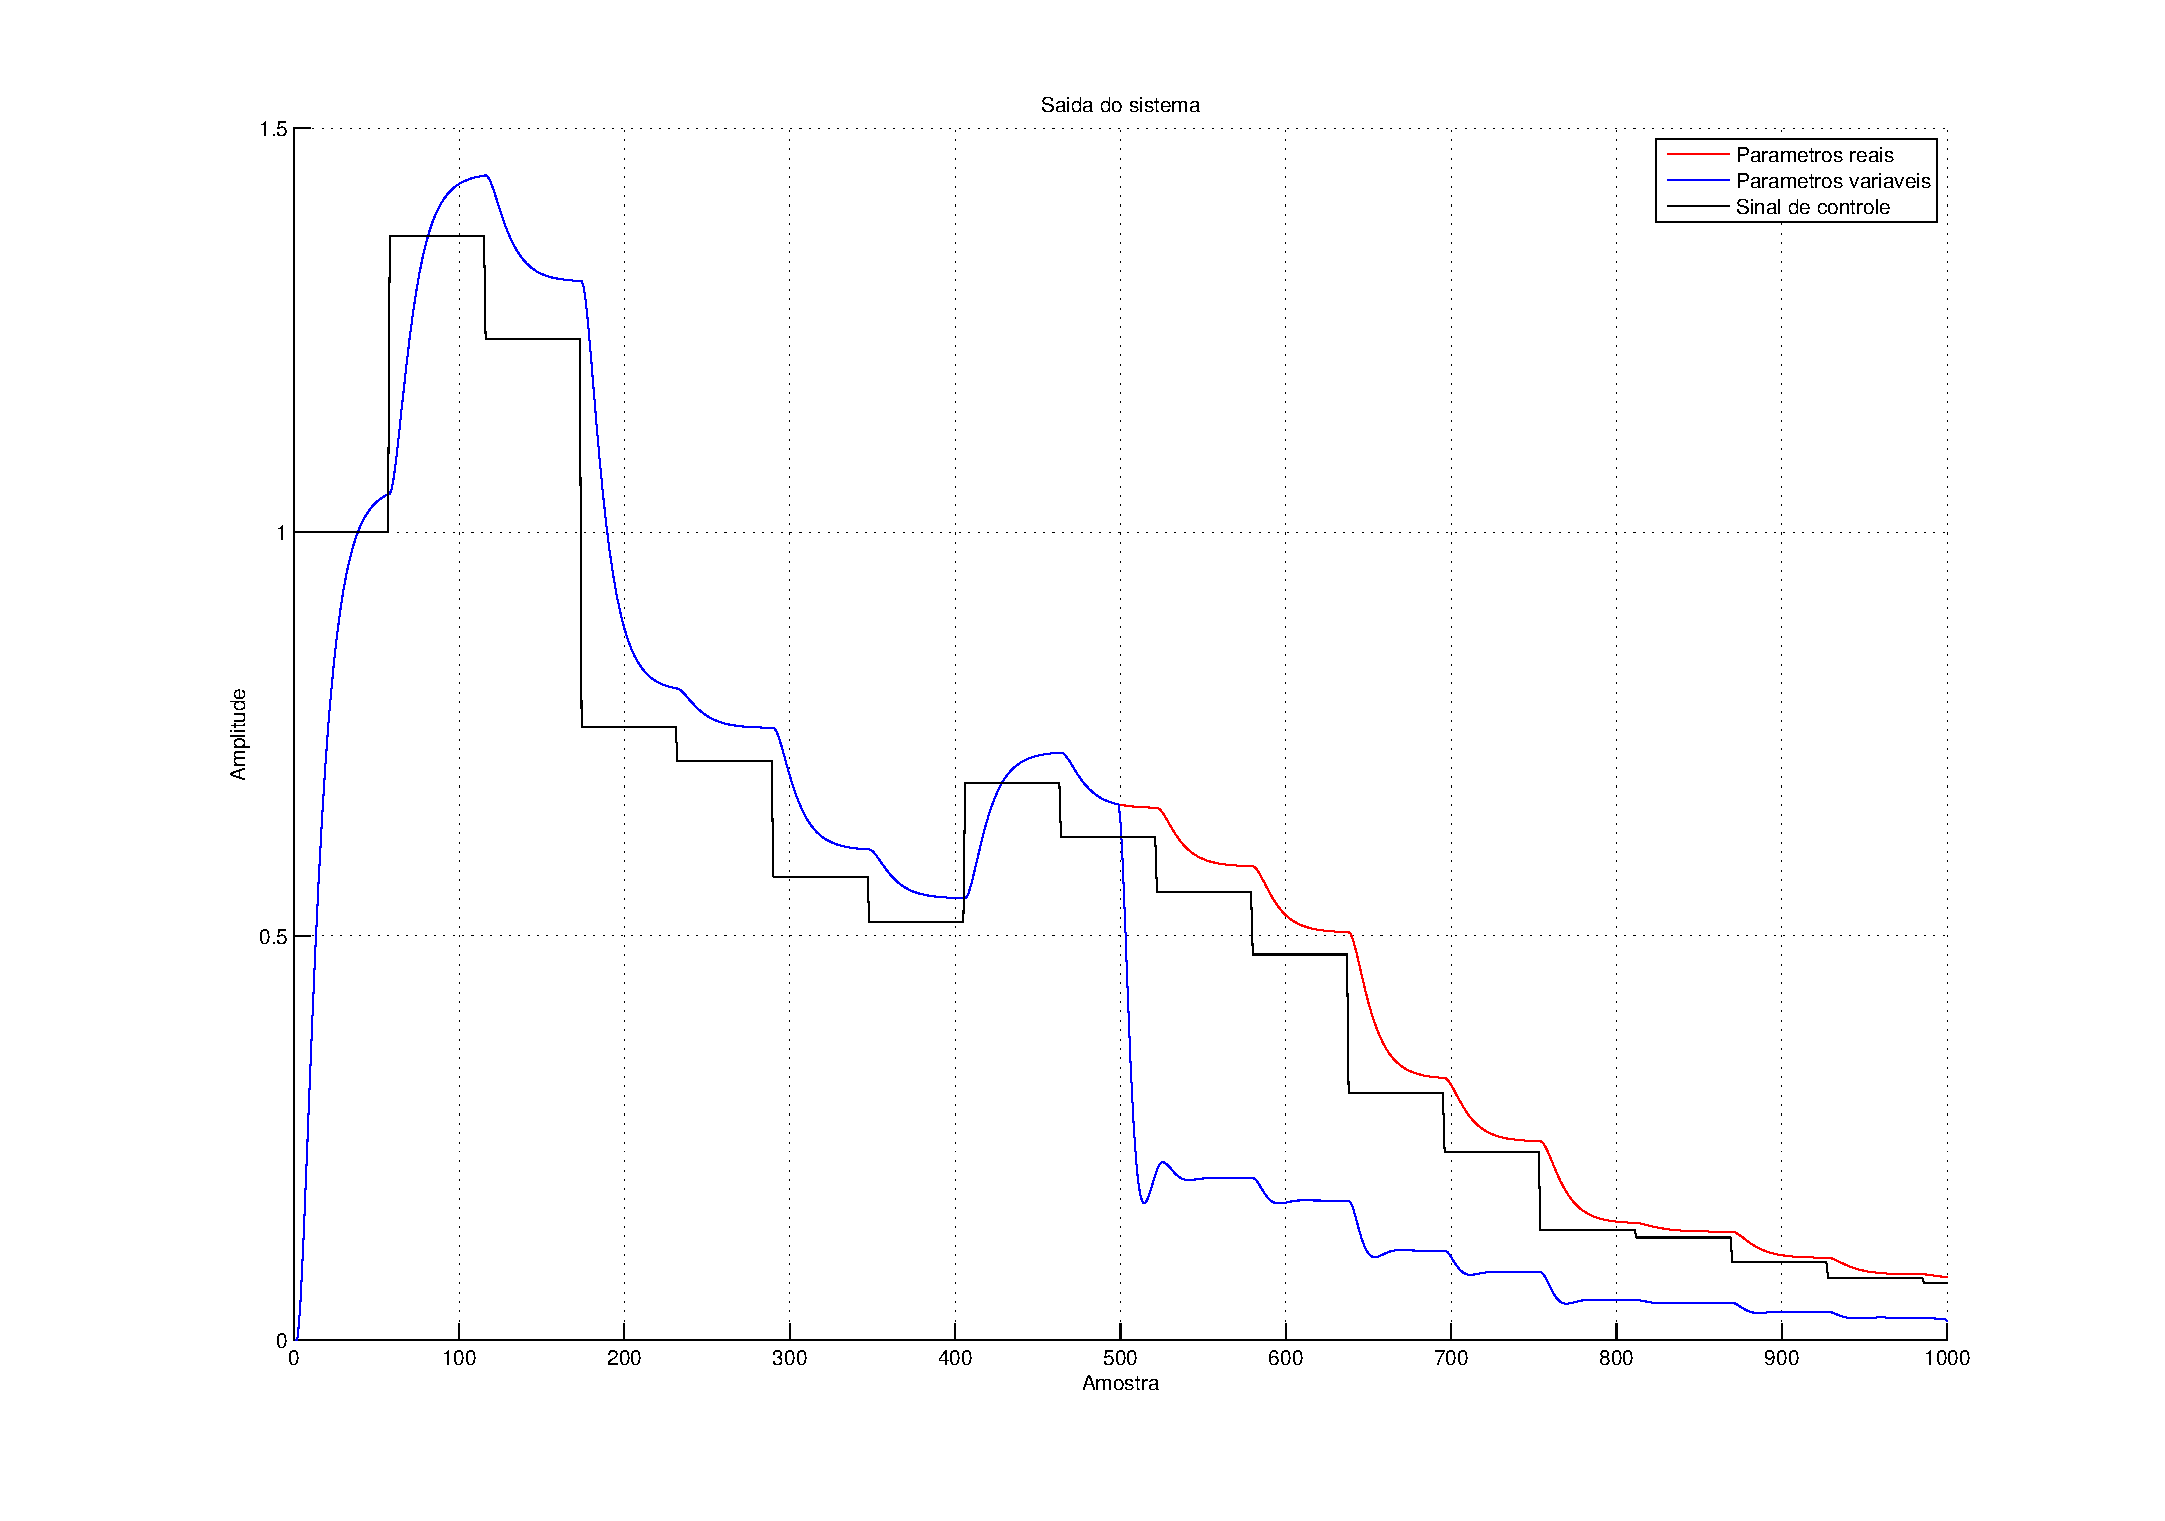
\includegraphics[width=0.95\textwidth]{imgs/questao2/saida_1000}
    \caption{Saída do sistema para $N = 1000$}
    \label{fig:saida_sist_1000}
\end{figure}

\begin{table}
\centering
    \caption{Estimativa realizada para $N = 1000$.}
    \label{tab:estimativa_1000}
    \vspace{0.25cm}
    \begin{tabular}{|c|c|c|c|}
        \hline
        Parâmetros & 
        $\mb{\theta}_{\text{ideal}}$&
        $\mb{\theta}_{\text{sem variação}}$&
        $\mb{\theta}_{\text{com variação}}$\\
        \hline
        \hline
        $a_1$ & $-1.724$   & $-1.7240$ & $-1.9613$ \\
        \hline
        $a_2$ & $0.7408$   & $0.7408$  & $0.9641$ \\
        \hline
        $b_1$ & $0.009056$ & $0.0096$  & $0.0100$ \\
        \hline
        $b_2$ & $0.008194$ & $0.0082$  & $-0.0073$ \\
        \hline
    \end{tabular}
\end{table}

Outra execução resultou em resultados semelhantes, como pode ser observado na
Fig. \ref{fig:saida_sist_1000_2} e na Tab. \ref{tab:estimativa_1000_2}

\begin{figure}[htb]
\centering
    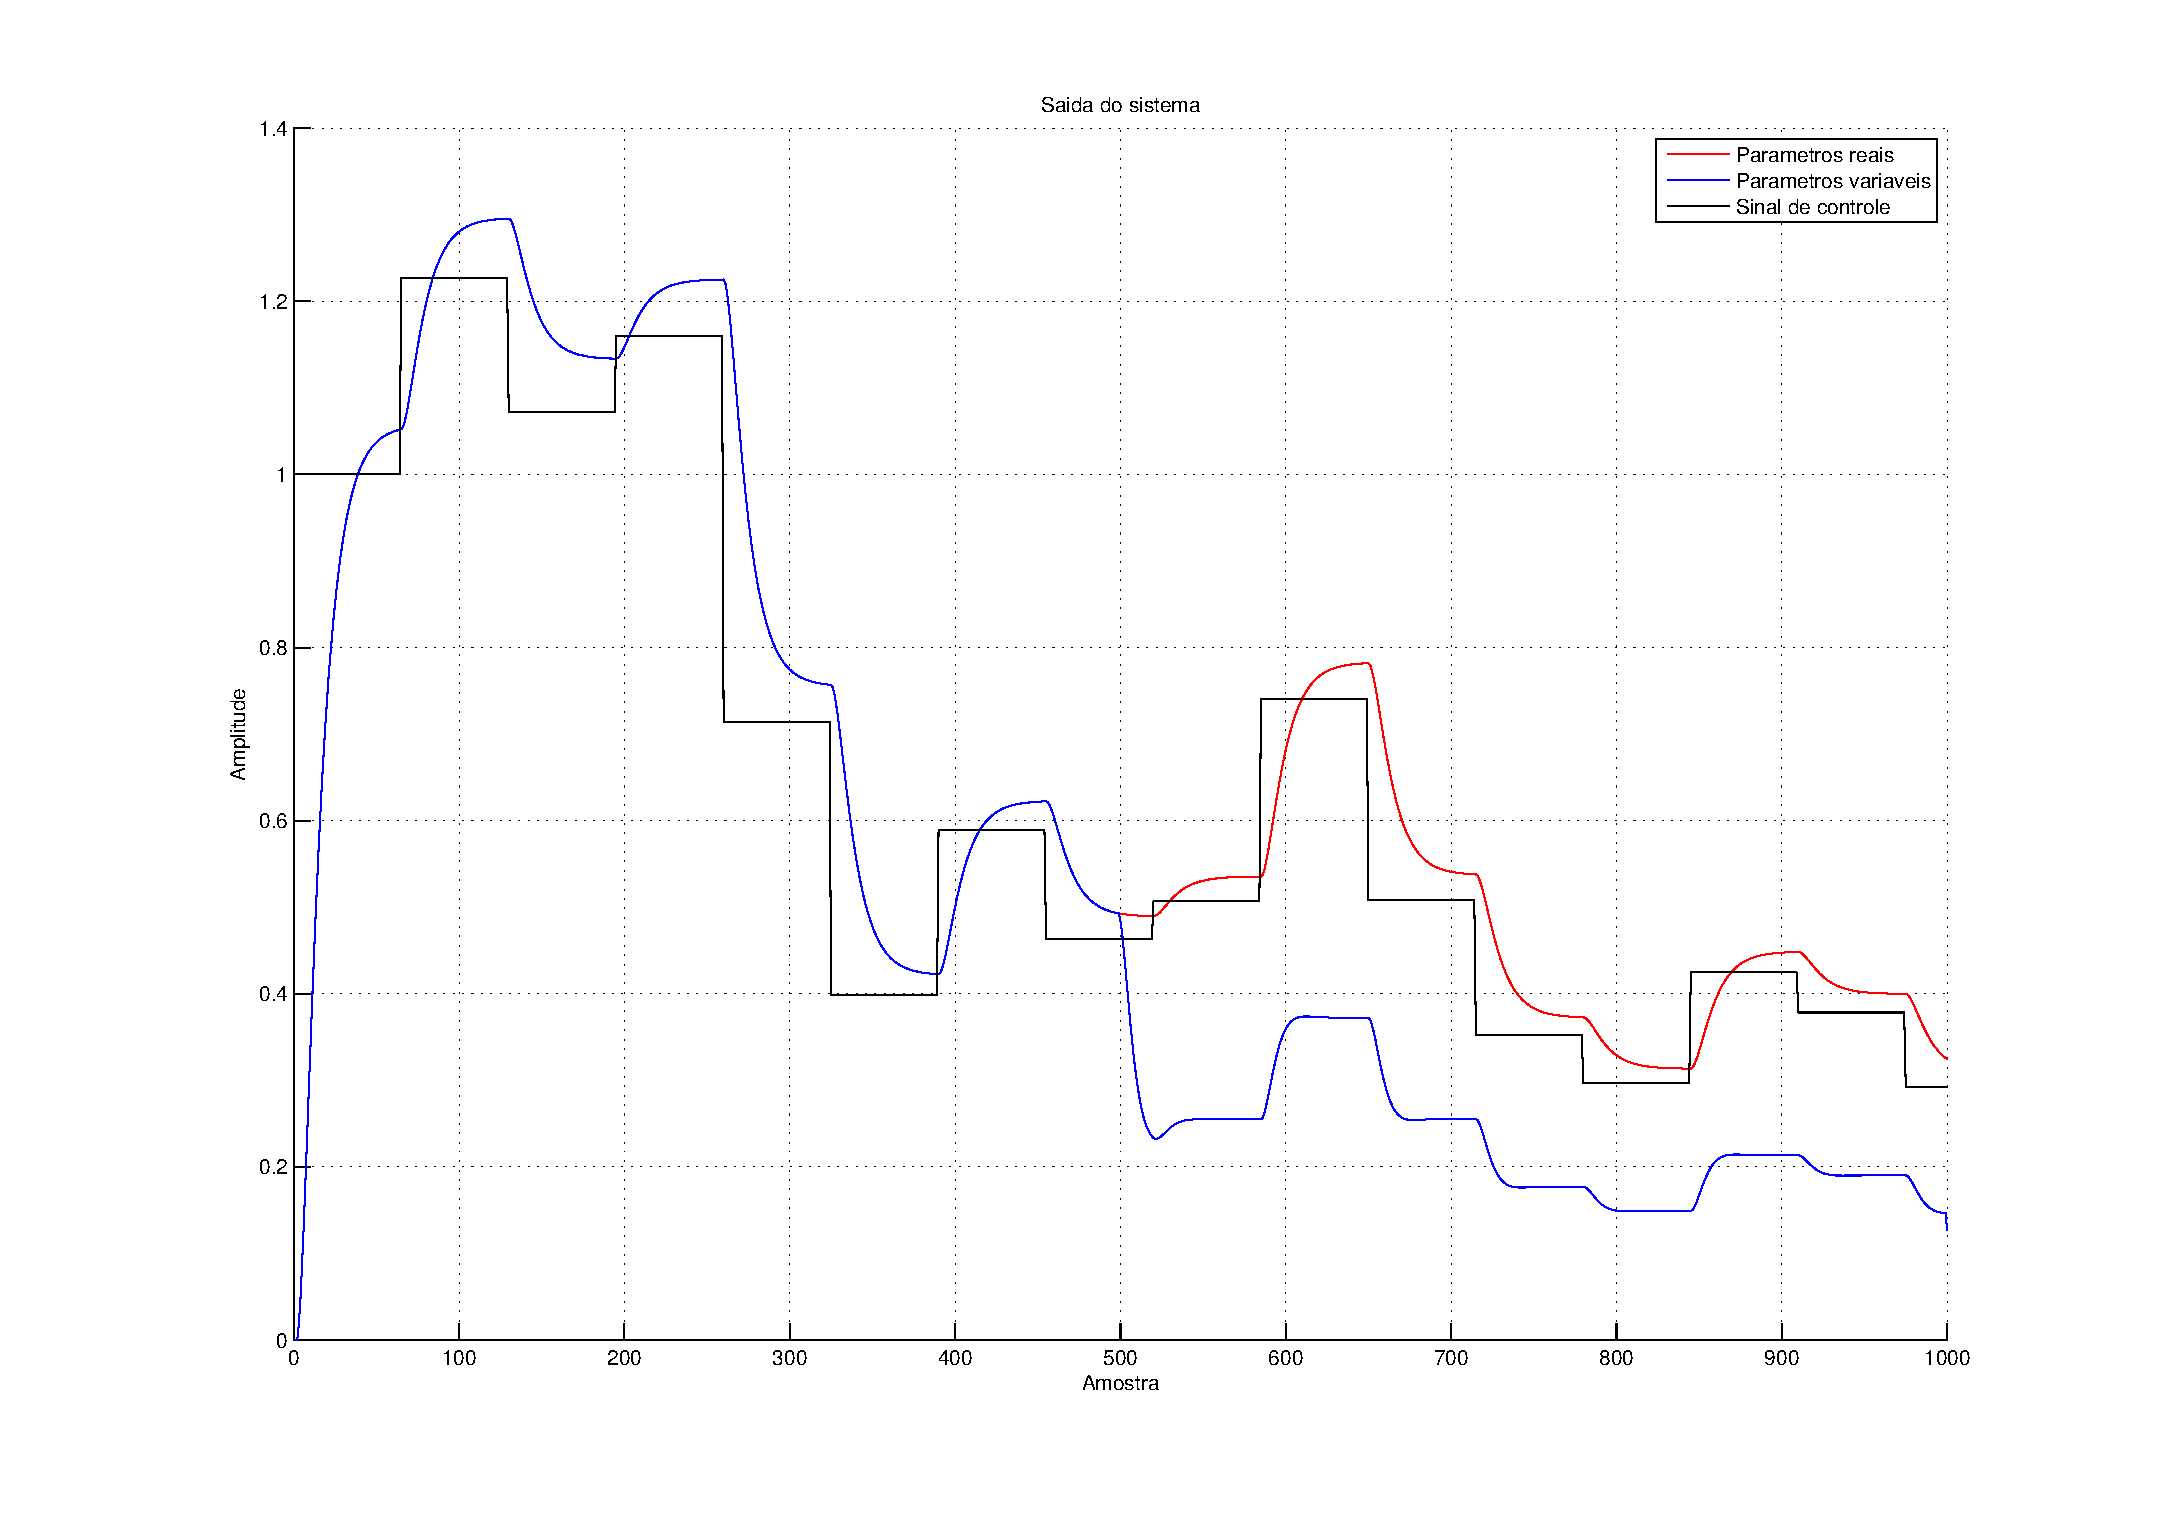
\includegraphics[width=0.95\textwidth]{imgs/questao2/saida_1000_2}
    \caption{Saída do sistema para $N = 1000$}
    \label{fig:saida_sist_1000_2}
\end{figure}

\begin{table}
\centering
    \caption{Estimativa realizada para $N = 1000$.}
    \label{tab:estimativa_1000_2}
    \vspace{0.25cm}
    \begin{tabular}{|c|c|c|c|}
        \hline
        Parâmetros & 
        $\mb{\theta}_{\text{ideal}}$&
        $\mb{\theta}_{\text{sem variação}}$&
        $\mb{\theta}_{\text{com variação}}$\\
        \hline
        \hline
        $a_1$ & $-1.724$   & $-1.7240$ & $-1.9661$ \\
        \hline
        $a_2$ & $0.7408$   & $0.7408$  & $0.9680$ \\
        \hline
        $b_1$ & $0.009056$ & $0.0096$  & $0.0093$ \\
        \hline
        $b_2$ & $0.008194$ & $0.0082$  & $-0.0076$ \\
        \hline
    \end{tabular}
\end{table}

Todos os valores aleatórios obtidos nas simulações seguiam uma distribuição
uniforme. O {\it script} do Matlab\textsuperscript{\textregistered} desenvolvido
para a resolução dessa questão pode ser encontrado no Apêndice \ref{ap:cod_q2}.
